\chapter{Introduction \\
\small{\textit{-- Author Name}} 
\index{Chapter!introduction}
\index{introduction}
\label{Chapter::Introduction}}

% Add a section and label it so that we can reference it later
\section{My Section \label{Section::MySection}}

All projects should have a small introduction.  Here we provide some
example LaTeX commands.  The first one is an example on how to
introduce a PNG file as an image into the document, together with 
how to use a cite, such as this one \cite{GM1998}.

\begin{figure}
\centering
\scalebox{0.8}{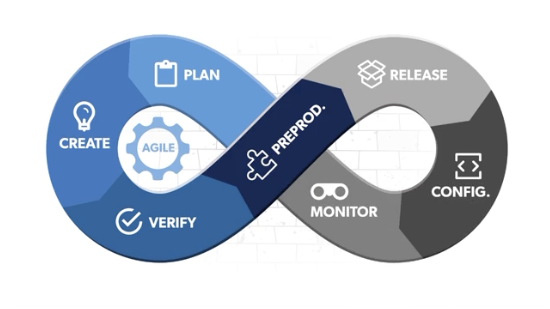
\includegraphics{Figures/manAgileProcess.png}}
\caption{\label{Figure::manAgile} Figure of the continuous agile process.}
\end{figure}

% add a new page
\newpage

Hi there world!  Here is an example of a note\footnote{Here is a reference 
to Figure \ref{Figure::manAgile} and an indexed keyword\index{keyword}.}

\section{Testing EPS Files}

%\begin{figure}
%\psfrag{a }{\hspace{-0.8in}\large \begin{tabular}{c} Memory \\ Data \end{tabular}}
%%\psfrag{b }{$\F^h = \lcb \bx \in \R^n: F_i(\bx) = f_i,  \forall i \rcb$}
%\psfrag{b }{$\sum_{i=0}^{N} x_i$}
%\centering
%\scalebox{1}{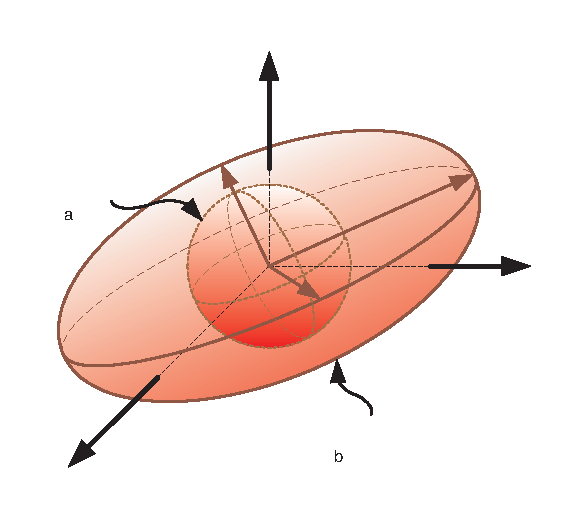
\includegraphics{Figures/manDenoise.eps}}
%\caption{\label{Figure::manDenoise} Showing an EPS file with PSFRAG.  The EPS file was created in Visio 2000.
%Note that the EPS file has letters 'a' and 'b' for the location that we want to replace.}
%\end{figure}